        \documentclass[margin,line]{resume}
 
\usepackage[latin1]{inputenc}
\usepackage[english,french]{babel}
\usepackage[T1]{fontenc}
\usepackage{fontawesome}
\usepackage{graphicx,wrapfig}
\usepackage{url}
\usepackage[colorlinks=true, pdfstartview=FitV, linkcolor=blue, citecolor=blue, urlcolor=blue]{hyperref}
\pdfcompresslevel=9


\begin{document}{\sc \Large Curriculum Vitae -- Alejandro Buren}
\begin{resume}

% === PICTURE ===

    \vspace{0.5cm}
    \begin{wrapfigure}{R}{0.15\textwidth}
         \vspace{-0.9cm}
        \begin{center}
        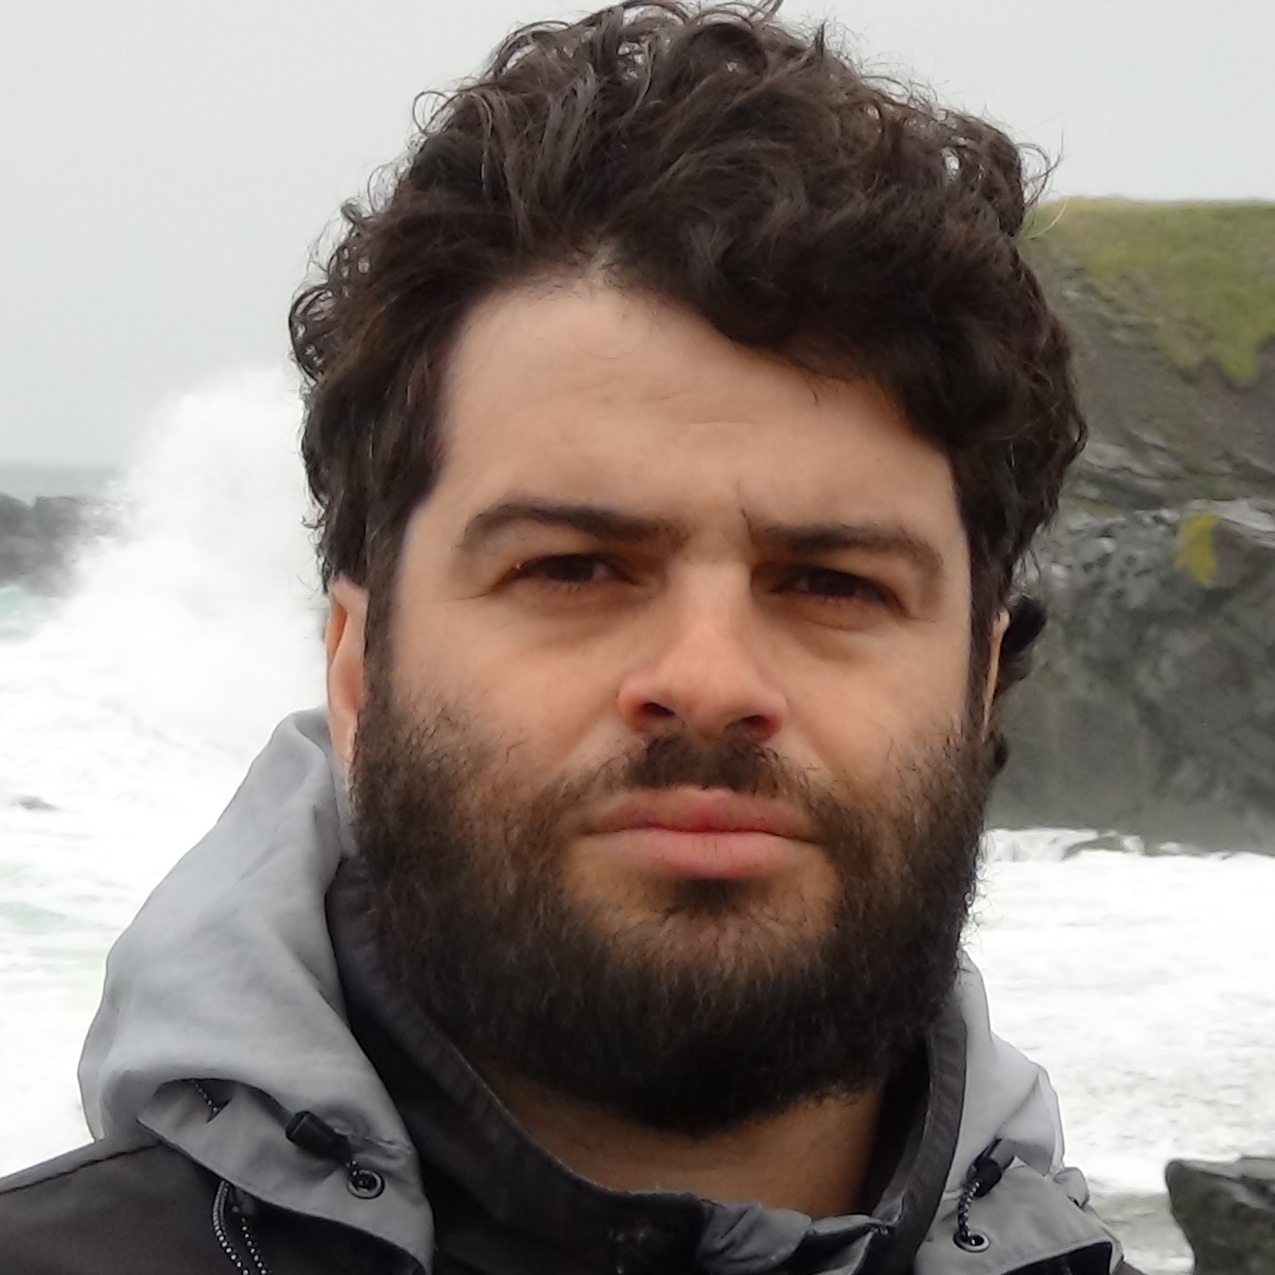
\includegraphics[width=0.15\textwidth]{Buren_profile.png}
        \end{center}
         \vspace{-1cm}
    \end{wrapfigure}

% === PERSONAL INFO ===
 
    \section{\mysidestyle Personal\\Information}
    Alejandro Buren \\
    Limoges, France\\ 
  %  \faTv  \space \href{http://www.microwave.fr}{www.microwave.fr} \\ 
    \faTwitter  \space \href{https://twitter.com/reveyrand/}{@reveyrand} \\
  %  \faLinkedin \space \href{http://www.linkedin.com/in/reveyrand/}{www.linkedin.com/in/reveyrand} \\ 
  %  \faYoutubePlay  \space \href{https://www.youtube.com/c/tibaultreveyrand/}{www.youtube.com/c/tibaultreveyrand}
   
% === OBJECTIVE ===

    \section{\mysidestyle Professional Objective}
    Improve the efficiency of the microwave and RF designers and structures. I focus on nonlinear devices at circuits level (such as HEMTs transistors) and at system level (HPA, Switches). That purpose requires an original use of an advanced RF instrumentation associated to a strong knowledge in terms of measured devices modeling.
 
% === SKILLS ===
       
    \section{\mysidestyle Skills}\vspace{2mm}       
    \begin{description}
            \item[Operating systems:] DOS, Windows, Unix and Linux.
                \item[Programming languages:] Pascal, 80x86 Assembler, C, C++, TCL/TK, JAVA, PHP, mySQL.
                \item[Office softwares:] Microsoft Office, Open Office, LaTeX, DocBook.
                \item[Scientific softwares] Comsys, Maple, Matlab, Mathematica, Scilab, Keysight's VEE and ADS, NI LabVIEW.
                \item[Characterization tools:] Spectrum analyzers, scopes, AWG, VNA, LSNA, probe stations, high impedance probes. I have developed calibration procedures and automated calibration and measurements processes.
                \item[System Level Modeling:] Amplifiers, modulators and mixers with splines, neural networks or Volterra expansions. Bilateral Modeling by PhD model.
                \item[Circuit Level Modeling:] Linear, nonlinear and electrothermal models of HEMTs.
                \item[Languages:] French, English.
    \end{description}
     
% === CERTIFICATIONS ===
    
      \section{\mysidestyle Certifications}
      \textbf{National Instruments} Certified LabVIEW Associate Developer (CLAD) \hfill \textsl{July 2014-July 2016}\\

% === AWARDS ===

      \section{\mysidestyle Awards}\vspace{4mm}  
      \begin{list2}
        \item \textbf{Best Paper Award}, European Microwave Week - Galium Arsenide Application Symposium (GAAS), 2002 \\
        \textsl{\footnotesize{T. Reveyrand, C. Maziere, J.M. N\'ebus, R. Qu\'er\'e, A. Mallet, L. Lapierre, J. Sombrin, ``A calibrated time domain envelope measurement system for the behavioral modeling of power amplifiers'', European Microwave Week, GAAS 2002, pp. 237-240, Milano, September 2002}}
        \vspace{1mm}
        \item \textbf{Best Student Paper Award}, Journ\'ees Nationales Micro-ondes (JNM), 2007 \\
\textsl{\footnotesize{
O. Jardel, F. De Groote, T. Reveyrand, C. Charbonniaud, J.P. Teyssier, R. Qu\'er\'e, D. Floriot, ``Mod\'elisation du drain-lag dans les mod\`eles \'electriques grand-signaux de transistors HEMTs AlGaN/GaN'', 15eme Journ\'ees Nationales Micro-ondes (JNM),3C1, Toulouse, Mai 2007.}}
      \end{list2}
        
        Up to 130 other refrences are available here : \\ 
        \vspace{-8mm}

\href{http://www.microwave.fr/publications.html}{http://www.microwave.fr/publications.html}
    %\vspace{-1mm}
    
% === ORGANIZATIONS ===

        \section{\mysidestyle Professional Organizations}%\vspace{2mm}       
          \textbf{The Institute of Electrical and Electronics Engineers (IEEE)}\\
          Member of:
          \begin{list2}
          \item{``Microwave Theory and Techniques'' society  \hfill \textsl{2007-present}}
          \item{``Instrumentation and Measurement'' society  \hfill \textsl{2007-present}}
          \item{MTT-11 ``Microwave Measurements'' technical committee \hfill \textsl{2009-present}}
          \item{IEEE MTT-S Technical Program Review Committee (TPRC) for IMS  \hfill \textsl{2013-present}}
          \item{Judge for IEEE MTT-S Graduate Fellowships  \hfill \textsl{2014-present}}
          \item{Chair for IEEE Denver Section Jt. Chapter, AP03/MTT17  \hfill \textsl{2015-2016}}
          
          \end{list2}
       \textbf{The European Microwave Association (EuMA)}\hfill \textsl{2009-2015}
       
       
       
       
       
       
       
       
        \vfill
       
    
    
% === HISTORY ===

        \section{\mysidestyle Employment History}\vspace{2mm}          
       
              
       \begin{description}
       
        
            \item[Measurement Engineer (CNRS)]\small{XLIM \hfill \textsl{June 2016-Present}}\\     
            \item[Lecturer]\small{University of Colorado, Boulder \hfill \textsl{January 2016-May 2016}}\\
                    ECEN 5014-003, ``Microwave Measurements and Calibration Fundamentals''
            \vspace{2mm}
                        
            \item[Research Associate]\small{University of Colorado at Boulder \hfill \textsl{June 2013-May 2016}}\\
            Achievements:
                \begin{list2}
                        \item{LabVIEW software for a ``Do-it-yourself'' Large-Signal Network Analyzer (LSNA)}
                        \item{Time domain measurement setup in Scilab (VTD-SWAP)}
                        \item{Outphasing PA characterizations}
                        \item{Load-pull in time-domain}
                    \end{list2}     
            \vspace{2mm}
 
   
            \item[Measurement Engineer (CNRS)]\small{XLIM \hfill \textsl{December 2007-May 2013}}\\
            Achievements:
                \begin{list2}
                        \item{Korrigan European Project activities (RTP N$^{\circ}$102.052 funded within the EUROPA framework in the CEPA2 priority area - ends early 2009) : GaN HEMTs circuits level modeling from european foundries (Thales / QinetiQ) for HPA, LNA and Switches}
                        \item{Time domain measurement setup (LSNA) development on Scilab-TCL/TK (GUI, calibration and measurement automation)}
                        \item{Development of HEMTs modeling tools (Scilab)}
                        \item{Contractual measurements such as load-pull, linearity, high impedance probe in both frequency (VNA) and time domain (LSNA)}
                    \end{list2}   
            \vspace{2mm}
            
                
            \item[Research Associate - Visiting Scholar]\small{University of Colorado at Boulder \hfill \textsl{February 2012-July 2012}}\\
                    GaN HEMTs based rectifiers characterizations and analysis
            \vspace{2mm}
                
            \item[Research Engineer (CNRS)]\small{XLIM \hfill \textsl{May 2005-November 2007}}\\
            Achievements:
            \begin{list2}
                \item{Frequency domain load-pull measurement setup (VNA in receiver mode with pulse capabilities) developpemnt with Scilab (calibration procedures, measurement automation, data processing)}
                \item{Large signal caracterization of transistor (mainly european GaN in the framework of Korrigan}
                \item{Korrigan WP3.3 workpackage leader in Korrigan. Developpement of a internet database (Php / mySQL) to let partners share data and informations}
                \item{GaN HEMTs ``spice-like'' nonlinear models}
            \end{list2}           
            \vspace{2mm}
            
            
            \item[Research Engineer]\small{NMDG Engineering bvba \hfill \textsl{November 2004-February 2005}}\\
                Implementation of the High Impedance Probe module (calibration and measurements) in the commercial LSNA Software (based on Mathematica)
 
            \vspace{2mm}
            
            
            \item[Postdoctoral scientist]\small{CNES (French Space Agency) \hfill \textsl{October 2003-September 2004}}\\
                Development of characterization tools interfaces within the free open-source scientific package Scilab
 
            \vspace{2mm}
            
            
            \item[Postdoctoral scientist]\small{CNES (French Space Agency) \hfill \textsl{October 2002-September 2003}}\\           
                    Achievements:
            \begin{list2}
                \item{Large Signal Network Analysis (LSNA) characterizations in time-domain}
                \item{Development of a new LSNA module in order to investigate time domain waveforms at internal nodes of MMICs with high impedance probes (HIP) to validate circuits designs and to analyze nonlinear parametric stability}
                \item{Large Signal Network Analysis (LSNA) characterizations in time-domain}
            \end{list2}           
            \vspace{2mm}
            
            
            \item[Researcher]\small{IRCOM / University of Limoges \hfill \textsl{October 1998-September 2002}}\\            
                    Achievements:
            \begin{list2}
                \item{Development of the RF time-domain envelope measurement setup (hardware and software)}
                \item{Development of the calibration procedure of the time-domain envelope measurement setup}
                \item{Power amplifiers characterizations : Load-pull, IM3, NPR}
                \item{Behavioral modeling of nonlinear devices with memory effects for system level}
                \item{Development of a dynamic complex gain model with neural networks}
            \end{list2}           
            \vspace{2mm}
            
            
            \item[Lecturer]\small{University of Limoges \hfill \textsl{October 1998-September 2002}}\\
                    RF devices, analog/digital communication systems, signal processing, propagation waves...
            \vspace{2mm}
            
            
            \item[Postgraduate student]\small{IRCOM / University of Limoges \hfill \textsl{February 1998-July 1998}}\\
                    Circuits level simulations of IM3 and NPR in order to optimize the trade-off between linearity and efficiency
                    
    \end{description}
    
    
       
      \section{\mysidestyle Education} 
       Ph.D in High Frequency Devices and Circuits - Electronic and Optoelectronic, April 2002 \\
      University of Limoges (France)       
           
\end{resume}   
\end{document}